% generated by scripts/pkl_to_latex.py
% source PKL : excited_singlet_v1_L6_Ne6_U10_t1_mode-uniform_tpall_t2all_tperpall_nmin2_solver-gcg_sz0_restarts10_iter200_kmax4_tol1em09_cut10_adaptive1_step5_clusteravg1_T0.01to5_N30-c4bc7f804a4c_k12_diag0.pkl
% scan type  : excited_singlet
% state      : ex_singlet
% requires   : \usepackage{pgfplots} \pgfplotsset{compat=1.18}
% colours match the matplotlib PDF (tab10 cycle)
\definecolor{gmeC0}{HTML}{1F77B4}
\definecolor{gmeC1}{HTML}{FF7F0E}
\definecolor{gmeC2}{HTML}{2CA02C}
\definecolor{gmeC3}{HTML}{D62728}
\definecolor{gmeC4}{HTML}{9467BD}
\definecolor{gmeC5}{HTML}{8C564B}
\definecolor{gmeC6}{HTML}{E377C2}
\definecolor{gmeC7}{HTML}{17BECF}

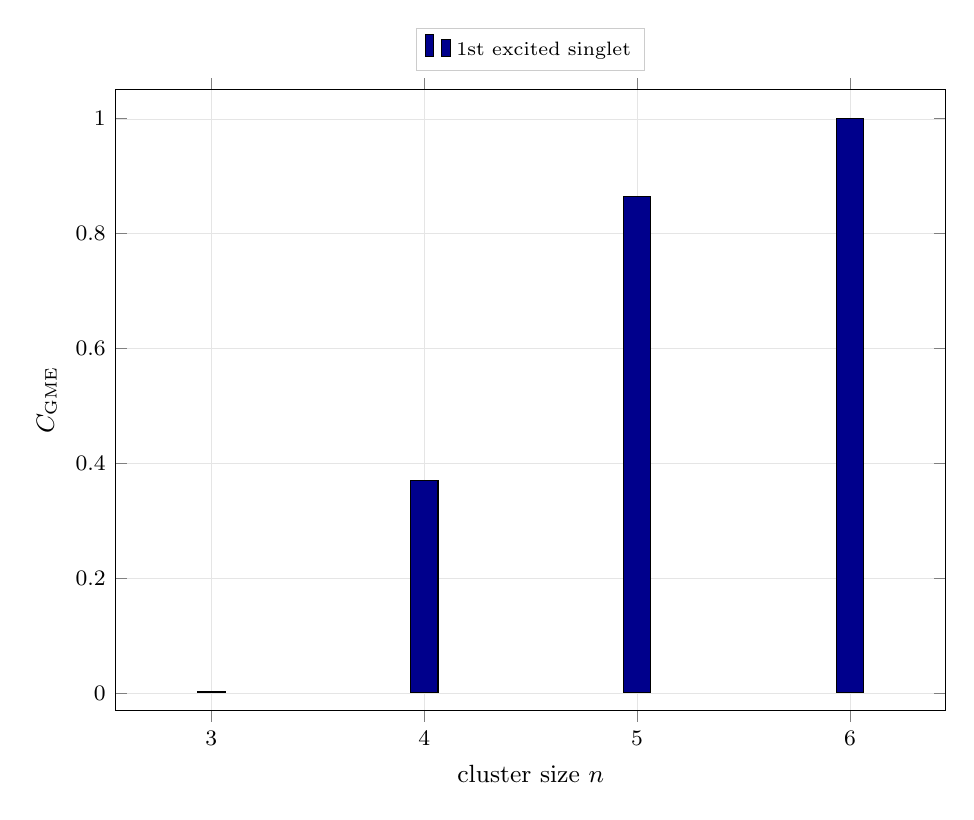
\begin{tikzpicture}
  \begin{axis}[
    width=\columnwidth,
    height=0.78\columnwidth,
    xlabel={cluster size $n$},
    ylabel={$C_{\mathrm{GME}}$},
    grid=both,
    grid style={line width=.1pt, draw=gray!20},
    tick label style={font=\footnotesize\rmfamily, /pgf/number format/fixed},
    label style={font=\small\rmfamily},
    scaled ticks=false,
    legend style={font=\scriptsize\rmfamily, draw=gray!40, at={(0.5,1.03)}, anchor=south, /tikz/every even column/.append style={column sep=6pt}},
    legend cell align={left},
    legend columns=1,
    ymin=-0.03,
    ymax=1.05,
    xtick={3,4,5,6}, ybar, enlarge x limits=0.15,
  ]
    \addplot[ybar, fill=blue!55!black, draw=black, bar width=10pt] coordinates {(3,0.003019) (4,0.370446) (5,0.864713) (6,1)};
    \addlegendentry{1st excited singlet}
  \end{axis}
\end{tikzpicture}

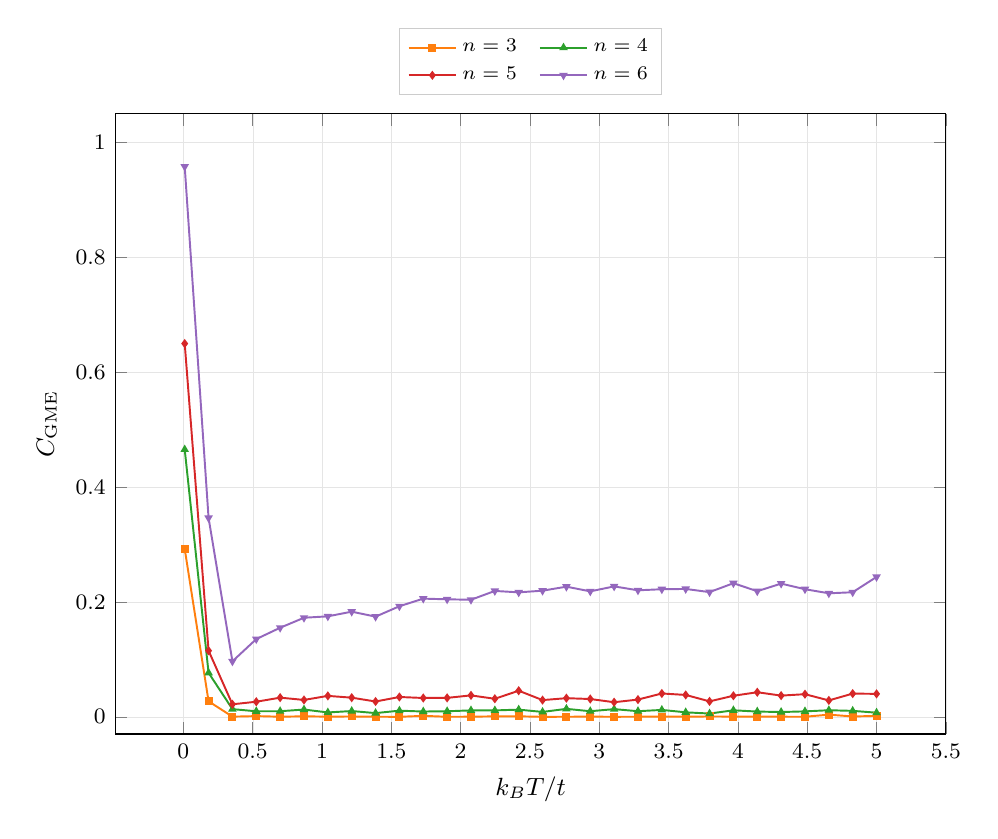
\begin{tikzpicture}
  \begin{axis}[
    width=\columnwidth,
    height=0.78\columnwidth,
    xlabel={$k_B T/t$},
    ylabel={$C_{\mathrm{GME}}$},
    grid=both,
    grid style={line width=.1pt, draw=gray!20},
    tick label style={font=\footnotesize\rmfamily, /pgf/number format/fixed},
    label style={font=\small\rmfamily},
    scaled ticks=false,
    legend style={font=\scriptsize\rmfamily, draw=gray!40, at={(0.5,1.03)}, anchor=south, /tikz/every even column/.append style={column sep=6pt}},
    legend cell align={left},
    legend columns=2,
    ymin=-0.03,
    ymax=1.05,
  ]
    \addplot[color=gmeC1, mark=square*, mark size=1.1pt, line width=0.7pt] coordinates {
        (0.01,0.292503) (0.182069,0.026992) (0.354138,0.000285) (0.526207,0.001219)
        (0.698276,0.000166) (0.870345,0.000864) (1.042414,0.000278) (1.214483,0.00058)
        (1.386552,0.00008) (1.558621,0.00002) (1.73069,0.001663) (1.902759,0.000071)
        (2.074828,0.000196) (2.246897,0.00078) (2.418966,0.000832) (2.591034,0.000004)
        (2.763103,0.000079) (2.935172,0.000328) (3.107241,0.000009) (3.27931,0.000148)
        (3.451379,0.000348) (3.623448,0.000187) (3.795517,0.000582) (3.967586,0.000388)
        (4.139655,0.000247) (4.311724,0.000174) (4.483793,0.000111) (4.655862,0.003785)
        (4.827931,0.00056) (5,0.001581)
    };
    \addlegendentry{$n=3$}
    \addplot[color=gmeC2, mark=triangle*, mark size=1.1pt, line width=0.7pt] coordinates {
        (0.01,0.465524) (0.182069,0.076685) (0.354138,0.01337) (0.526207,0.009637)
        (0.698276,0.009726) (0.870345,0.012652) (1.042414,0.007588) (1.214483,0.010055)
        (1.386552,0.006449) (1.558621,0.0107) (1.73069,0.009192) (1.902759,0.009663)
        (2.074828,0.011183) (2.246897,0.01114) (2.418966,0.01249) (2.591034,0.008497)
        (2.763103,0.013836) (2.935172,0.009727) (3.107241,0.013366) (3.27931,0.009771)
        (3.451379,0.011992) (3.623448,0.007821) (3.795517,0.005662) (3.967586,0.011339)
        (4.139655,0.009119) (4.311724,0.008341) (4.483793,0.009462) (4.655862,0.011441)
        (4.827931,0.010363) (5,0.007157)
    };
    \addlegendentry{$n=4$}
    \addplot[color=gmeC3, mark=diamond*, mark size=1.1pt, line width=0.7pt] coordinates {
        (0.01,0.649933) (0.182069,0.115093) (0.354138,0.021806) (0.526207,0.026244)
        (0.698276,0.033355) (0.870345,0.029381) (1.042414,0.03643) (1.214483,0.033336)
        (1.386552,0.026657) (1.558621,0.034499) (1.73069,0.032791) (1.902759,0.032973)
        (2.074828,0.037307) (2.246897,0.031396) (2.418966,0.045427) (2.591034,0.029109)
        (2.763103,0.032439) (2.935172,0.030984) (3.107241,0.025387) (3.27931,0.030007)
        (3.451379,0.040628) (3.623448,0.038083) (3.795517,0.026895) (3.967586,0.036671)
        (4.139655,0.042784) (4.311724,0.036937) (4.483793,0.039387) (4.655862,0.028532)
        (4.827931,0.040431) (5,0.03997)
    };
    \addlegendentry{$n=5$}
    \addplot[color=gmeC4, mark=triangle*, mark size=1.1pt, mark options={rotate=180}, line width=0.7pt] coordinates {
        (0.01,0.958182) (0.182069,0.346305) (0.354138,0.096626) (0.526207,0.135371)
        (0.698276,0.155093) (0.870345,0.172514) (1.042414,0.17496) (1.214483,0.183089)
        (1.386552,0.174425) (1.558621,0.192528) (1.73069,0.205791) (1.902759,0.204623)
        (2.074828,0.203843) (2.246897,0.219182) (2.418966,0.216737) (2.591034,0.219638)
        (2.763103,0.226614) (2.935172,0.218467) (3.107241,0.227106) (3.27931,0.220292)
        (3.451379,0.222165) (3.623448,0.222658) (3.795517,0.217139) (3.967586,0.232641)
        (4.139655,0.218719) (4.311724,0.23197) (4.483793,0.222202) (4.655862,0.215091)
        (4.827931,0.216903) (5,0.24361)
    };
    \addlegendentry{$n=6$}
  \end{axis}
\end{tikzpicture}

\begin{table}[htbp]
  \centering
  \caption{Spin classification of the lowest eigenstates of the $L=6$, $K=6$ Hubbard ring.}
  \label{tab:spin-l6-ne6-f7477b}
  \begin{tabular}{rrrrrl}
    \hline\hline
    Index & Energy & $\langle S^2\rangle$ & $S$ & $2S+1$ & Label \\
    \hline
    0 & -1.664363 & -0.0000 & 0.00 & 1 & Singlet (S=0) \\
    1 & -1.390497 & 2.0000 & 1.00 & 3 & Triplet (S=1) \\
    2 & -1.163673 & -0.0000 & -0.00 & 1 & Singlet (S=0) \\
    3 & -1.080001 & 2.0000 & 1.00 & 3 & Triplet (S=1) \\
    4 & -1.080001 & 2.0000 & 1.00 & 3 & Triplet (S=1) \\
    5 & -0.967248 & 2.0000 & 1.00 & 3 & Triplet (S=1) \\
    6 & -0.967248 & 2.0000 & 1.00 & 3 & Triplet (S=1) \\
    7 & -0.781279 & 0.0000 & 0.00 & 1 & Singlet (S=0) \\
    8 & -0.781279 & -0.0000 & -0.00 & 1 & Singlet (S=0) \\
    9 & -0.771276 & 6.0000 & 2.00 & 5 & Quintet (S=2) \\
    10 & -0.582576 & 6.0000 & 2.00 & 5 & Quintet (S=2) \\
    11 & -0.582576 & 6.0000 & 2.00 & 5 & Quintet (S=2) \\
    \hline\hline
  \end{tabular}
\end{table}
